% !TEX program = lualatex
% !TEX options = -synctex=1 -interaction=nonstopmode -file-line-error -shell-escape -output-directory=%OUTDIR% "%DOC%"

\documentclass[12pt, a4paper]{article}
\usepackage{amsfonts}
\usepackage{amssymb}
\usepackage{amsmath}
\usepackage[english]{babel}
\usepackage{caption}
\usepackage{float}
\usepackage[left=2cm, top=2cm, right=2cm, bottom=2cm]{geometry}
\usepackage{graphicx}
\usepackage{listings}
\usepackage[newfloat, outputdir=.texcache]{minted}
\usepackage{pgf}
\usepackage{pdfpages}

\graphicspath{{figures/}}

\setlength\parindent{0pt}

\newcounter{lstNoteCounter}
\SetupFloatingEnvironment{listing}{name=Source code}


\begin{document}
  \centerline{\Huge\scshape Computational physics}
  \vspace*{0.5cm}
  \hrule
  \vspace*{0.5cm}
  \centerline{Jona Ackerschott, Julian Mayr}
  \vspace*{1cm}
  \centerline{\Large\bfseries Problem set 8}
  \vspace*{0.5cm}

  \section*{Problem 1}
  A plot of the characteristic polynomial for different values of $r$ is given below (see source code \ref{source_problem1_python1}).
  \begin{figure}[h]
    \centering
    \resizebox{\textwidth}{!}{
      \input{figures/fig1.pgf}
    }
    \caption{Plots of the characteristic polynomial $P(\lambda)$ for 4 equidistant values for $r$ between 0.0 (blue graph) and 1.8 (red graph)}
  \end{figure}

  The zeros of $P(\lambda)$ are computed with the mathematica method \texttt{NRoots} as well as exported and plotted in python (see source code \ref{source_problem1_mathematica} and \ref{source_problem1_python2}). The result is given below

  \begin{figure}[h]
    \centering
    \resizebox{\textwidth}{!}{
      \input{figures/fig2.pgf}
    }
    \caption{Zeros of the characteristic polynomial $P(\lambda)$, plotted in the complex plane, for $r$ from approximately 1.34561 to 28 in steps of 1}
  \end{figure}

  Interpretation of the results is skipped here, due to time constraints.

  \newpage
  \captionsetup{type=listing}
  \inputminted{mathematica}{problem1.txt}
  \caption{Mathematica input for problem 1}
  \label{source_problem1_mathematica}

  \captionsetup{type=listing}
  \inputminted{python}{problem11.py}
  \caption{Python code for problem 1}
  \label{source_problem1_python1}

  \captionsetup{type=listing}
  \inputminted{python}{problem12.py}
  \caption{Python code for problem 1}
  \label{source_problem1_python2}

  \newpage
  \section*{Problem 2}
  Using the scipy-builtin RK45 solver, the solution of the Lorenz attractor problem was computed numerically for different values of r. The initial condition y0 was chosen to be $(0.1, 0.1, 0.1)$ + the chosen fixed Point. The solutions were 3d-plotted with matplotlib.
  

  \begin{figure}
    \centering
	  \includegraphics[width=0.75\textwidth]{{r=0.5000}.pdf}
    \caption{$r=0.500$}
  \end{figure}
  
  \begin{figure}
    \centering
	  \includegraphics[width=0.75\textwidth]{{r=1.1500}.pdf}
    \caption{$r=1.150$}
  \end{figure}
  
  \begin{figure}
    \centering
	  \includegraphics[width=0.75\textwidth]{{r=1.3456}.pdf}
    \caption{$r=1.3456$}
  \end{figure}
  
  \begin{figure}
    \centering
	  \includegraphics[width=0.75\textwidth]{{r=24.0000}.pdf}
    \caption{$r=24.000$}
  \end{figure}
  
  \begin{figure}
    \centering
	  \includegraphics[width=0.75\textwidth]{{r=28.0000}.pdf}
    \caption{$r=28.000$}
  \end{figure}
  
  For the stable values of r, the solutions converge oscillating aroud the nearest fix point (stable solutions). For the higher values, they move around it chaotically without ever converging (chaotic solutions). 

  Next, for r=27 and y0 as chosen in a), a stable solution, the z cordinate of the local minima in z of the solution were plotted against the previous z value. This plot converges  against the Point $(30,30)$ on the diagonal, so $z=30$. The slope of the funtion is less than 1, so the point seems to be stable, as the z coordinate also converges.

  \begin{figure}
    \centering
    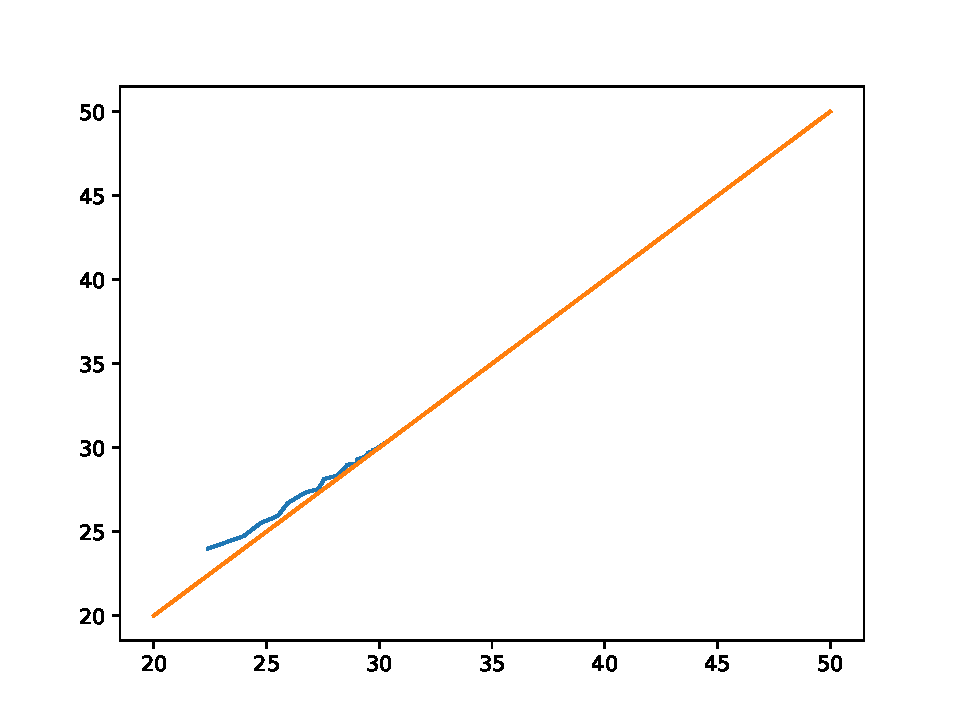
\includegraphics[width=0.75\textwidth]{zk.pdf}
    \caption{$z_k(z_{k+1}$ plotted from $k=4$ to $k=100$}
  \end{figure}


  \begin{figure}
    \captionsetup{type=listing}
    \inputminted{python}{problem2.py}
    \caption{Mathematica input for problem 2}
  \end{figure}
  

\end{document}
